%%%%%%%%%%%%%%%%%%%%%%%%%%%%%%%%%%%%%%%%%%%%%%%%%%%%%%%%%%%%%%%%%%%%%%%%%%%%%%%%
% FUENTE
%%%%%%%%%%%%%%%%%%%%%%%%%%%%%%%%%%%%%%%%%%%%%%%%%%%%%%%%%%%%%%%%%%%%%%%%%%%%%%%%

% Plantilla creada por Eduardo Mosqueira Rey a partir de un original de
% Rational Software Corporation

%%%%%%%%%%%%%%%%%%%%%%%%%%%%%%%%%%%%%%%%%%%%%%%%%%%%%%%%%%%%%%%%%%%%%%%%%%%%%%%%
% CONFIGURACIÓN TEXSTUDIO DEL CORRECTOR ORTOGRÁFICO
%%%%%%%%%%%%%%%%%%%%%%%%%%%%%%%%%%%%%%%%%%%%%%%%%%%%%%%%%%%%%%%%%%%%%%%%%%%%%%%%

% !TeX spellcheck = es_ES
% Usar el lenguaje es_ES para la corrección en castellano

%%%%%%%%%%%%%%%%%%%%%%%%%%%%%%%%%%%%%%%%%%%%%%%%%%%%%%%%%%%%%%%%%%%%%%%%%%%%%%%%
% TIPO DE DOCUMENTO Y PAQUETES
%%%%%%%%%%%%%%%%%%%%%%%%%%%%%%%%%%%%%%%%%%%%%%%%%%%%%%%%%%%%%%%%%%%%%%%%%%%%%%%%

\documentclass[12pt, a4paper, titlepage]{article}

\usepackage[spanish]{babel} % Soporte multilenguaje para LaTeX.
\usepackage[a4paper, top=2.5cm, bottom=2.5cm, left=2.5cm, right=2.5cm]{geometry} % Interfaz flexible para definir las dimensiones del documento
\usepackage[utf8]{inputenc} % Aceptar diferentes tipos de codificación de caracteres de entrada (en este caso usamos la codificación Unicode UTF-8)
\usepackage{graphicx} % Soporte aumentado para gráficos 
\usepackage{color} % Para usar colores
\usepackage{hyperref} % Para manejar referencias cruzadas. P.ej. añadir hiperenlaces al índice


\begin{document}

%%%%%%%%%%%%%%%%%%%%%%%%%%%%%%%%%%%%%%%%%%%%%%%%%%%%%%%%%%%%%%%%%%%%%%%%%%%%%%%%
% PORTADA
%%%%%%%%%%%%%%%%%%%%%%%%%%%%%%%%%%%%%%%%%%%%%%%%%%%%%%%%%%%%%%%%%%%%%%%%%%%%%%%%

\begin{titlepage}


\includegraphics[width=15cm]{Imagenes/Simbolo_logo_UDC.png}

% Lista de tamaños: \Huge, \huge, \LARGE, \Large, \large, \small, \footnotesize, \tiny
\vspace{6cm}

\begin{flushright}

	\LARGE{\textbf{Monitorización de pruebas}}
	
	\large{\textbf{VVS}}
\end{flushright}

\vspace{3cm}
\begin{center}
	\large{\textbf{Historial de revisiones}}
	
    \begin{tabular}{ | p{3cm} | p{2cm} | p{4cm} | p{6cm} |}
    \hline
    \textbf{Fecha} & \textbf{Versión} & \textbf{Descripción} & \textbf{Autores} \\ \hline
     16/12/2015 &  1.0 &  Ejercicio de refactorización & Xoán Andreu Barro Torres \newline F. Javier Moure López \newline Emma Oitavén Carracedo \\ \hline
    \end{tabular}
\end{center}

\end{titlepage}
\clearpage

%%%%%%%%%%%%%%%%%%%%%%%%%%%%%%%%%%%%%%%%%%%%%%%%%%%%%%%%%%%%%%%%%%%%%%%%%%%%%%%%
% INDICE
%%%%%%%%%%%%%%%%%%%%%%%%%%%%%%%%%%%%%%%%%%%%%%%%%%%%%%%%%%%%%%%%%%%%%%%%%%%%%%%%

\tableofcontents
\newpage

%%%%%%%%%%%%%%%%%%%%%%%%%%%%%%%%%%%%%%%%%%%%%%%%%%%%%%%%%%%%%%%%%%%%%%%%%%%%%%%%
\section{Contexto}

Este documento hace referencia a las pruebas realizadas sobre el proyecto de la asignatura VVS llamado Spoticopy\footnote{https://github.com/andreu-barro/VVS} encontrado en el repositorio de GitHub.

\section{Estado actual}

Listaxe de funcionalidades actuais, as súas especificacións, as persoas responsables do seu desenvolvemento, e as persoas responsables do proceso de proba.  Para cada funcionalidade: número de probas obxectivo, número de probas preparadas, porcentaxe executada e porcentaxe superada. Se esta información é profusa e se almacena noutra fonte, referencia á fonte. Se é cambiante, referencia a unha \emph{shapshot} ou resumo do mais destacado.

\section{Registro de pruebas}
\subsection{JUnit}
JUnit se utiliza para realizar pruebas unitarias sobre nuestra aplicación, nos sirven para encontrar errores y solventar los problemas en la programación de forma manual.
Se realizan pruebas de todas las funciones implementadas en la aplicación.
\subsection{Quickcheck}
QuickCheck es una implementación de la herramienta de prueba basada especificación QuickCheck .
El objetivo de QuickCheck es sustituir los valores recogidos manualmente con los valores generados . Una prueba basada en QuickCheck trata de cubrir las leyes de un dominio , mientras que la prueba clásica sólo puede probar la validez de los valores distintos. Es una mejora de Junit y podemos encontrar problemas de rendimiento con las iteraciones. \\
Se crean generadores de:
\begin{itemize}
	\item GeneradorContenido
	\item GeneradorCancion
	\item GeneradorServidor
	\item GeneradorServidorVacio
\end{itemize}

Con estos generadores, se comprueban las funciones de Servidor normal y que todo está funcionando correctamente.

\subsection{Cobertura}
Realizada la prueba de cobertura de pruebas, se observa que faltan muchos test por implementar, por lo que se procede a implementar los test que faltan, según la información que nos ofrece el plugin de ecobertura.\\
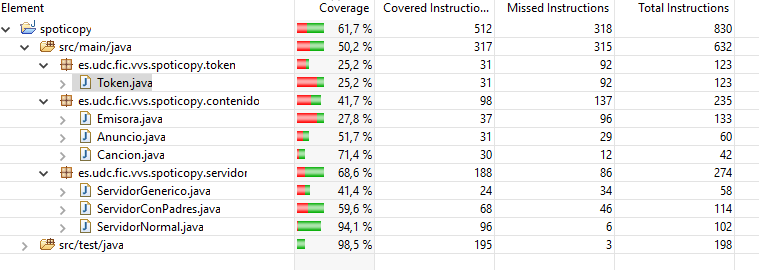
\includegraphics[width=15cm]{Imagenes/CoberturaSemana1.png} \\

Después de:
\begin{itemize}
	\item Aumentar cobertura de Anuncio (casi al 100%)
	\item Aumentar cobertura de ServidorNormal (al 100%)
	\item Aumentar cobertura de ServidorGenerico (casi al 100%)
	\item Aumentar cobertura de Token 
	\item Aumentar cobertura de ServidorConPadres
\end{itemize}

Quedó:

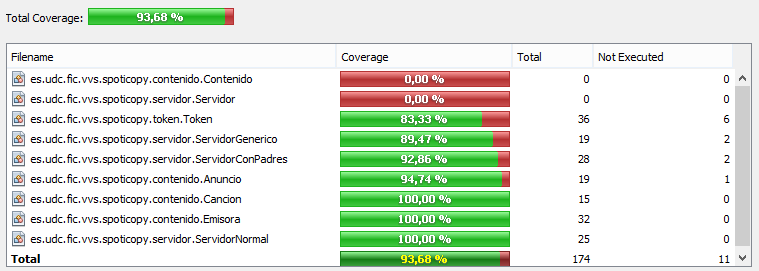
\includegraphics[width=15cm]{Imagenes/CoberturaSemana2.png} \\

\subsection{PIT (mutation testing)}

Realizado el mutation testing, resultados:

\href{Informes/PIT1/index.html}{Informe PIT} \\

\subsection{FindBugs}

FindBugs es un programa que utiliza el análisis estático para buscar errores en el código de Java.

En la versión inicial podemos comprobar que tenemos los siguientes errores:
\href{Informes/SiteTestInicial/findbugs.html}{Informe Find bugs} \\

\section{Registro de errores}

Todos los errores localizados, modificaciones necesarias, etc. pueden encontrarse referenciados en el documento de CHANGELOG.txt, en el cual se encuentran las correcciones hasta el momento.


\section{Estadísticas}

\begin{itemize}
	\item Errores diarios encontrados:
	\item Errores semanales encontrados:
	\item Progreso en las pruebas:
	\item Análisis del perfil de detección de errores (lugares, componentes, tipología).
	\item Informe de errores abiertos y cerrados por nivel de criticidad.
	\item Evaluación global del estado de calidad y estabilidad actuales.
\end{itemize}

\section{Otros aspectos de interés}

Nada de momento. Se conserva el apartado para el futuro.

\end{document}